%%%%%%%%%%%%%%%%%%%%%%%%%%%%%%%%%%%%%%%%%%%%%%%%%%%%%%%%%%%%%%%%%%%%%%%%%%%%%%%%
%
%   Semester project, fall term 2014
%   Author: Jakob Ehrl, born 01/24/91
%   Study program: Computer science, MA 1
%   
%   Professor Dr. Francesco Mondada
%   Assistant: Dr. Stefan Witwicki
%
%%%%%%%%%%%%%%%%%%%%%%%%%%%%%%%%%%%%%%%%%%%%%%%%%%%%%%%%%%%%%%%%%%%%%%%%%%%%%%%%%

\chapter{Introduction}
The MarXbot is a ground robot moving on so-called ``treels'' (a combination of tracks and wheels). It is equipped with a gripper arm that can be rotated around the main body. The gripping mechanism itself is a magnet, which can attach to magnetic objects if activated. In prior work, various controllers have been developed that enable the robot to approach, align with and pick up objects following a finite state machine. The objective of this semester project was to apply reinforcement learning in a way that the robot would learn from one of the pre-programmed controllers and improve the desired behavior using a learning algorithm. Proper alignment between the robot and the object is crucial for being able to pick up an object. Therefore, we targeted the behaviors of the robot from approaching an object to aligning its gripper with the object surface.

\chapter{Methods}

\section{Hardware}
Until now, there is no simulation available that mimics the capacities and behaviors of the MarXbot. Therefore, both development and testing was performed directly on the MarXbot in a prepared environment.

\subsection{The MarXbot}
\begin{figure}
    \centering
    \def\svgwidth{0.5 \textwidth}
    \input{figures/marxbot.pdf_tex}
    \caption{Scematic drawing of the MarXbot}
    \label{fig:marxbot_scematic}
\end{figure}

\figurename~\ref{fig:marxbot_scematic} shows the schematic assembly of the MarXbot. A two-dimensional perspective on the robot is adequate for all following explanations as there will be no motion along the $z$-axis. The gripper is kept at a constant height.
Locomotion is based on differential actuation of the two treels. A treel is hereby a combination of a track and a wheel placed next to the track. The gripper can rotate $360^\circ$ around the main body. An array of ten equally spaced infrared (IR) sensors (denoted by $s_0$ -- $s_9$) in the front of the magnet allow for distance measurements.

All sensors and actuators form separate modules. Each module is controlled by its respective  micro-controller. Executed on the micro-controllers therefore runs in a parallel fashion. Most relevant for this work are the modules controlling the gripper (gripper-main and gripper-front) and the treels (treel-left and treel-right). Additionally, the robot disposes of a unix-based computer that allows for interfacing via WiFi and also for the execution of programs that take a higher level of control over the modules.
This description of the MarXbot is not complete but covers the relevant parts for this context.

\subsection{Target}
As our general objective, we defined the alignment between robot and object. Hereby, the object is a cube made of styrofoam. Its dimensions are 6~cm $\times$ 6~cm $\times$ 6~cm. However, the robot's perception of objects is not accurate due to interference and ray bending. Hence, for a given sensor snapshot, small objects seem round to the robot even though they have straight edges. Therefore, we require our styrofoam block to cover at least four IR sensors when placed directly in front of the gripper.

\subsection{Test Environment}
A specifically designed arena served as testing environment. The floor is made of wood and is even over the whole arena. Walls around the arena prevent the robot from escaping.

%\begin{itemize}
%    \item MarXbot
%    \item Block
%    \item Arena
%    \item Computer
%\end{itemize}

\section{Software}
Software development was divided into two parts: low-level and high-level, where low-level means code that runs directly on the micro-controllers and high-level is everything that runs on the MarXbot main computer. High-level control (de-)activates the executions of low-level tasks.

\subsection{Low-Level, Aseba}

%\begin{itemize}
%    \item Original controller: \texttt{cube-mover} 
%    \item Adapted controller: \texttt{helper}
%    \item Interactive controller: \texttt{combined-learner}
%\end{itemize}

\subsubsection{Original controller: \texttt{cube-mover}}
\texttt{cube-mover} is a controller that guides the robot through a set of ``modes'' based on a finite state machine. Depending on the incoming event
the robot performs the cube alignment and picks up the cube or drops it at a chosen location. Sequential modes are:
1. \texttt{IDLE},
2. \texttt{APPROACHING},
3. \texttt{ROTATING\_RIGHT\_AROUND\_GRIPPER},
4. \texttt{ALIGNING\_LATERALLY},
5. \texttt{ROTATING\_LEFT\_AROUND\_GRIPPER},
6. \texttt{ALIGNING\_ANGLE},
7. \texttt{ALIGNING\_OFFSET},
8. \texttt{GRIPPING\_AND\_CARRYING\_CUBE},
9. \texttt{DROPPING\_CUBE}

%\begin{enumerate}
%    \item \texttt{IDLE}
%    \item \texttt{APPROACHING}
%    \item \texttt{ROTATING\_RIGHT\_AROUND\_GRIPPER}
%    \item \texttt{ALIGNING\_LATERALLY}
%    \item \texttt{ROTATING\_LEFT\_AROUND\_GRIPPER}
%    \item \texttt{ALIGNING\_ANGLE}
%    \item \texttt{ALIGNING\_OFFSET}
%    \item \texttt{GRIPPING\_AND\_CARRYING\_CUBE}
%    \item \texttt{DROPPING\_CUBE}
%\end{enumerate}

Out of these, modes 2 -- 7 cover the steps that are to be improved. Consequently, the goal is to learn a strategy that brings the robot in a good position to execute mode 8.

\subsubsection{Adapted controller: \texttt{helper}}
While \texttt{cube-mover} is performing modes 2 -- 7 it always adjusts its motor speeds depending on the actual actual distance to the cube and also the angle between gripper and cube. These almost continuous adjustments cannot be easily mapped to a finite action space. A small action space is desirable for the purpose of learning. Therefore, the original controller was modified such that rotational and translational movements are only performed at distinct motor speeds.

Another drawback of \texttt{cube-mover} is that modes 3 and 5 are performed while the gripper is raised above the robot body. Relying only on distance measurements coming from the gripper-front module, this means that the robot has no perception at all during modes 3 and 5. To overcome this problem, the gripper height is kept constant.

A controller following the state machine from above while drawing its actions only from the reduced action space was created as \texttt{helper}.

\subsubsection{Interactive controller: \texttt{combined-learner}}
In order to interact with the robot and advice particular actions (as sent from a remote-control or as learned from the learning algorithm), the controller \texttt{combined-learner} was developed. It implements two principles: Actions can be drawn from \texttt{helper} or be advised from a higher level via the even \texttt{take\_action}. Actions are performed at a fixed sampling rate of 0.3 seconds. When an action is advised from outside the \texttt{helper} controller is disabled via a flag but its state machine keeps running in order to continue at a later point when it is enabled again. As such, the initial autonomous controller can be used as a fall-back or even to strategically explore unknown states.

%TODO: anything about the synchronization here?

\subsection{High-Level, Python}

%\begin{itemize}
%    \item Action tracking: \texttt{logger}
%    \item Constrained actions: \texttt{actionControl}
%    \item Data processing and learning: \texttt{learner}
%    \item Remote-control
%\end{itemize}

\subsubsection{Action tracking: \texttt{logger}}
To track states and actions performed by the robot, the event \texttt{log\_update\_complete} was introduced. It consists of 19 entries and contains current IR sensor readings, line estimation parameters, gripper angle, motor speeds of gripper and treels and the type of the current action. This information is passed to the module \texttt{logger} where it is saved to a file. Action types encode the instance that advised an action, i.e. whether the action was drawn from the \texttt{helper} any of the higher levels (learned controller, random action, simple communication between \texttt{combined-learner} and \texttt{helper}).

\subsubsection{Constrained actions: \texttt{actionControl}}
Given that the target object is considerably light and the robot's force feedback does not detect collisions with the styrofoam block, proper alignment could be achieved by a simple strategy: ``Hit the block and keep going until it lies completely on the gripper.'' To avoid this mis-behavior in the learned policy we add constraints to the action space that forbid actions causing potential collisions.

Additional constraints are added to prevent the robot from losing the line of sight to the cube. There will never be a unique rule for the case where the block is not seen and therefore we cannot expect the robot to learn a policy for this special case. Technically, one could keep track of the last cube location at time $t_{i-1}$ but this would increase the state space with little benefit.

\subsubsection{Data processing and learning: \texttt{learner}}
The same information as given to the logging mechanism is fed to the module \texttt{learner}. There, it is translated into the respective states and actions. According to the new measurements, a value is computed for the last state-action pair. This belongs to the learning process.

Based on the learned experience, the learning algorithm computes a recommendation for the next action. In case there is no experience yet that covers the current state, an adequate action from a nearby known state can be used. This also encourages exploration. If the current state is a goal state this is indicated by recommending the action ``HALT''. The \texttt{learner} indicates when a state is completely new and thereby allows for exploration using the \texttt{helper} or executing random actions.


\section{Data Collection}
Final interaction with the robot was implemented in the script \texttt{combined-learner}. Together with the respective controller, this script allows for various options. One can either use \texttt{helper} exclusively, steer the robot manually via remote-control, let the \texttt{learner} act, perform random actions or specify a combination of these options. Measurements and executed actions are written to a log file.

%TODO more about synchronization here?

%\begin{itemize}
%    \item Helper
%    \item Remote-control
%    \item Learner
%    \begin{itemize}
%        \item $Q_{max}\left(s\right)$, if state $s$ is known
%        \item $Q_{max}\left(s_{N}\right)$, if neighbor state $s_{N}$ is known
%        \item random action
%    \end{itemize}
%\end{itemize}

\section{Learning Algorithm}

\subsection{Q-Learning}

Our learning algorithm uses Q-learning to learn an optimal policy. Q-learning assumes an underlying Markov Decision Process. It belongs to the class of model-free learning algorithms. This means that rather than learning a model of the world including transition tables and transition probabilities it directly learns values for actions given a particular state. Action-values are denoted by $Q(s_t, a_t)$, where $s_t$ is the observed state and $a_t$ is the action performed at time $t$. The $Q$-function updates and thereby gradually learns action-values through repeated experience according to Eq.~\eqref{eq:q}

\begin{equation}
    Q_{t+1}(s_t, a_t) = Q_t(s_t, a_t) + \alpha \cdot \left( R_{t+1} + \gamma \cdot \underset{a}{max} \: Q_t(s_{t+1}, a) - Q(s_t, a_t) \right),
    \label{eq:q}
\end{equation}

where $R_{t+1}$ is the immediate reward of action $a_t$ performed in state $s_t$. $\alpha \in \left(0,1\right]$ controls the impact of the new observation and $\gamma \in \left[0,1\right)$ controls how much future $Q$-values are valued. In order to apply Q-learning, an adequate representation of states and actions must be defined. Every time an action is executed, Eq.~\eqref{eq:q} is applied to the state the robot was in before executing the action.

\subsection{Representation of Actions}
Other than in \texttt{cube-mover}, only a distinct set of actions is available to the robot when working under learning conditions. All actions are performed at pre-defined speeds for time steps of 0.3 seconds. An action can be one of the following:

\begin{enumerate}
\setcounter{enumi}{-1}
    \item \textit{HALT}: all motors idle
    \item \textit{STEP\_FW}: both treels forward
    \item \textit{STEP\_BW}: both treels backward
    \item \textit{TURN\_L}: left treel backward, right treel forward
    \item \textit{TURN\_R}: left treel forward, right treel backward
    \item \textit{LOOK\_L}: gripper to the left
    \item \textit{LOOK\_R}: gripper to the right
    \item \textit{TWIST\_L}: \textit{TURN\_L} while \textit{LOOK\_R}
    \item \textit{TWIST\_R}: \textit{TURN\_R} while \textit{LOOK\_L}
\end{enumerate}

A sequence of actions 3 and 6 or 4 and 5 could lead to the same outcome as action 7 or 8 respectively. Therefore, the \textit{TWIST} actions are not strictly necessary. However, in order to leverage demonstrations from the \texttt{helper} more efficiently, they were added explicitly.

\subsection{Representation of States}
The direct measurements contain ten IR sensor readings as well as the angle between gripper and body. A measure for relative alignment between gripper and object must be computed from the IR readings. \texttt{cube-mover} estimates parameters for the line representing the cube surface as observed by the robot but fails when the cube is too close or only partly observable. A different parameter encoding the angular alignment was introduced:

Consider \figurename~\ref{fig:s_min_mu}. The object as observed by the robot is illustrated with black stripes. From robot-perspective, one can compute the object's center of mass as the centroid $\vec{\mu}$ of the visible area. The $y$-coordinate of the centroid is not of much interest as we do not know how deep the object is but the $x$-coordinate can still give us information about how well the cube is centered in front of the gripper. Together with the closest edge, it also allows allows to infer a rough approximation of the angle between gripper and block.

The representation of the current state includes the value and the sensor index of the closest measured distance $\vec{s_{min}}$, the gripper angle $\rho$ and the $x$-coordinate of the objects center of mass $\mu_x$. A state $s$ is then fully described by the tuple $s = \left(s_{min_x}, s_{min_y}, \mu_x, \rho \right)$. A state is considered a goal state if $\mu_x = 4.5$ (block centered) and at least 4 sensor readings are equal to $d_{opt}$.

\begin{figure}
    \centering
    \def\svgwidth{0.5 \textwidth}
    \input{figures/s_min_mu.pdf_tex}
    \caption{Visualization of the state parameters $\mu_x$ and $\vec{s_{min}}$ with the centroid of the observed area denoted as dot}
    \label{fig:s_min_mu}
\end{figure}

\subsubsection{Discretization of Distances and Angles}
\begin{figure}
    \centering
    \def\svgwidth{0.5 \textwidth}
    \input{figures/distances.pdf_tex}
    \caption{Distance discretization (values in mm)}
    \label{fig:distances}
\end{figure}

\figurename~\ref{fig:distances} illustrates discretization of the 2-D space that $\vec{s_{min}}$ can lie in. $s_{min_x}$ is the index of the IR sensor with the minimal distance measurement and can therefore only take values from 0 -- 9. $s_{min_y}$ is the respective distance measured at$s_{min_x}$. In favor of a smaller and more general state representation, this distance is discretized in the interval $[0,d_{max}]$ in steps of 5~mm. $d_{max}$ is the distance beyond which IR measurements become unreliable and was empirically defined as 120~mm. If all measurements are above $d_{max}$ the block is considered as not seen.

Angular measurements for $\rho$ lie within $\left[-90^\circ,90^\circ\right]$, where $\rho = 0^\circ$ denotes the angle when both treels and gripper are facing forward. This parameter is discretized in steps of $2^\circ$. $mu_x$ is discretized in steps of 0.5 (for cases where it lies between two sensors). The total number of possible states is approximately $4\times10^5$. Ignoring \textit{HALT} the complete state space grows to $3\times10^6$.

\subsection{Reward Function}
\begin{figure}
    \centering
    \def\svgwidth{0.5 \textwidth}
    \input{figures/reward.pdf_tex}
    \caption{Mapping from distances to state evaluation}
    \label{fig:reward}
\end{figure}

Referring back to Eq.~\eqref{eq:q} a reward function is needed to compute immediate feedback $R_{t+1}$ for performed actions. Our goal state was defined in terms of sensor measurements and their deviation from the goal distance. In the same way, we can evaluate each state in terms of distance measurements. The state evaluation shown in \figurename~\ref{fig:reward} assigns a value $r_i$ to each sensor measurement $d_i$, where $r_i \in [0,1]$. The total evaluation of a state is computed as $eval = \sum_{i} r_i$.

In a natural way, one could expect reward for improving the situation. Following this idea, we compute the direct reward as the difference between the last state and the current state that this action has lead to: $R_{t+1} = eval_{t+1} - eval_{t}$. Consequently, $R$ is not completely deterministic. Still, rewards can be expected to be similar when transitioning between two states multiple times and the computed $Q$ value will eventually involve average values for $R$.

\subsubsection{Alternative Representation of States}
After exhaustive testing, the robot did not seem to learn sufficiently well. One possible reason might have been the complex state representation and also the definition of goal states that allowed to declare some states as goal states in one episode and as non-goal states in other episodes. In order to improve the learning, the goal condition was changed to being a particular state (instead of depending on the current measurements). Also the state variable $\mu_x$ was exchanged to shrink the state space.

\figurename~\ref{fig:alternative} shows the changes in the state representation. $s_{min}$ is now determined after discretization. The highlighted area shows that sensors $s_5$ -- $s_7$ all fall into the same bin after discretization. The left-most sensor index is taken as new $s_{min_x}$ and $s_{min_y}$ is still the value of the corresponding bin (not changed). A new parameter, $line$, is computed from the number of sequential sensors with measurements in that same bin. It is now used to approximate the angular alignment. In this example, $line = -2$ as there are two additional sensors in the same bin and the right-most one of them measures a lower distance than the left-most one.

$line$ can take values in $[-3,3]$. If more than four sensors show measurements of $s_{min}$ only the left-most four are considered. The state $\left(s_{min_x} = 3, s_{min_y} = 45\:mm, \rho = 0^\circ, line = 3 \right)$ uniquely defines the goal.

Using this state representation, there are approximately $1\times10^5$ possible states. Consequently the size of the whole state-action space is reduced to $1\times10^6$. This representation was used for the following experimental evaluation.

\begin{figure}
    \centering
    \def\svgwidth{0.5 \textwidth}
    %\input{figures/alternative.pdf_tex}
    \input{figures/alternative_for_presentation.pdf_tex}
    \caption{Visualization of the alternative state parameters $\vec{s_{min}}$ and $line$ with the highlighted area as the interval of the closest discretized measurements}
    \label{fig:alternative}
\end{figure}



\chapter{Online-Learning and Experimental Evaluation}

\section{Experiments}
Several experiments were conducted to test and evaluate the developed controllers and the learning algorithm. Various initial distances between cube and gripper were tested.

\subsection{Training Episodes in Different Modes}
To gather experience that the robot could learn from, the following list of episodes was done.

%\begin{enumerate}
%    \item Helper only (13x)
%    \item Remote-control only (13x)
%    \item Combined learner (without random actions) and helper (23), occasional remote-control in the end of an episode
%    \item Learner with random exploration (at probability $p = 0.2$ and in case the encountered state is not known yet), occasional remote-control
%\end{enumerate}

\subsubsection{Debugging and Improving the \texttt{helper}}
A total of 47 episodes was carried out during an initial phase where the main purpose was on the proper implementation of the \texttt{helper} controller. For this heavily simplified version of \texttt{cube-mover} it was crucial to find the most appropriate motor speed parameters. Also the timing needed to be tuned in order to guarantee a synchronized execution of actions. Log data were collected throughout this phase and will be used to increase the robot's experience in a final phase.

\subsubsection{Experiment 1: \texttt{helper} only} 
After intensive testing, 13 episodes of exclusive \texttt{helper}-control followed. The objective of this phase was to explore various cube-robot configurations with pure guidance and thereby build up basis experience for the learning algorithm. Hence, log data from this phase serves the robot to learn from demonstration.

\subsubsection{Experiment 2: remote-control only}
The \texttt{helper} itself can only explore a limited number of state-action pairs given the underlying state machine. For instance, it would never do driving maneuvers while the gripper is not at $0^\circ$ or $90^\circ$. In order to make the robot aware of the advantage of smooth maneuvers similar to sideways parking, a series of 13 remote-controlled episodes was carried out. Data from this experiment is expected to optimize the trajectories and thereby the learned policy.

\subsubsection{Experiment 3: online-learning}
Building up on the experience from experiment 1, an initial Q-table was generated. During 23 episodes the robot would execute actions as recommended by the \texttt{learner} or call the \texttt{helper}. The policy was to leverage knowledge from the existing entries in the Q-table. If the encountered state was not known, the \texttt{learner} would search for a neighboring state that is similar in terms of geometry (individual state variables only vary within a small range). Only in cases where neither the state nor a neighboring state were found the \texttt{helper} is called to demonstrate. Once the \texttt{learner} is able to recommend actions again the \texttt{helper} is disabled.

The Q-table is updated in real time and the experience of successive episodes accumulates.

\subsubsection{Experiment 4: random exploration}
Similar to experiment 3, this experiment is based on the initial experience after experiment 1. It contains 14 episodes. Other than in experiment 3, actions are not always given by the \texttt{learner} or \texttt{helper} but are executed at random $20\%$ of the time. This allows the learning algorithm to explore state-action pairs that are not known yet and probably would not be executed otherwise. 

Having a constant probability of random exploration, the robot is not guaranteed to reach a goal state at all and episodes take longer than in the other experiments. After an execution time of 20 minutes, episodes were stopped manually. To make the robot succeed in at least some of the episodes manual remote-control was added occasionally.

\subsubsection{Experiment 5: standardized configurations}
A set of robot-cube configurations was created to evaluate the learned policy and the original \texttt{cube-mover} performance. 

\subsection{Cube-Robot Configurations}
A test set of 18 configurations was designed to compare the original controller, the modified one and the learned one. For each scenario, the initial location and orientation of both robot and cube were drawn on paper (see \figurename~\ref{fig:plan}). This ensures that all the controllers are given the same starting conditions. The initial distance between cube and gripper was 8~cm.

The six angular offsets were: $0^\circ$ (\textbf{Z}ero), $-15^\circ$ (\textbf{N}egative \textbf{L}ow), $-30^\circ$ (\textbf{N}egative), $15^\circ$ (\textbf{P}ositive \textbf{L}ow), $30^\circ$ (\textbf{P}ositive), $45^\circ$ (\textbf{E}xtreme).

The three lateral offset positions were: cube centered in front of IR array (\textbf{C}enter), cube on the right side of the IR array (\textbf{R}ight), cube on the left side of the IR array (\textbf{L}eft).

\begin{figure}
	\centering
	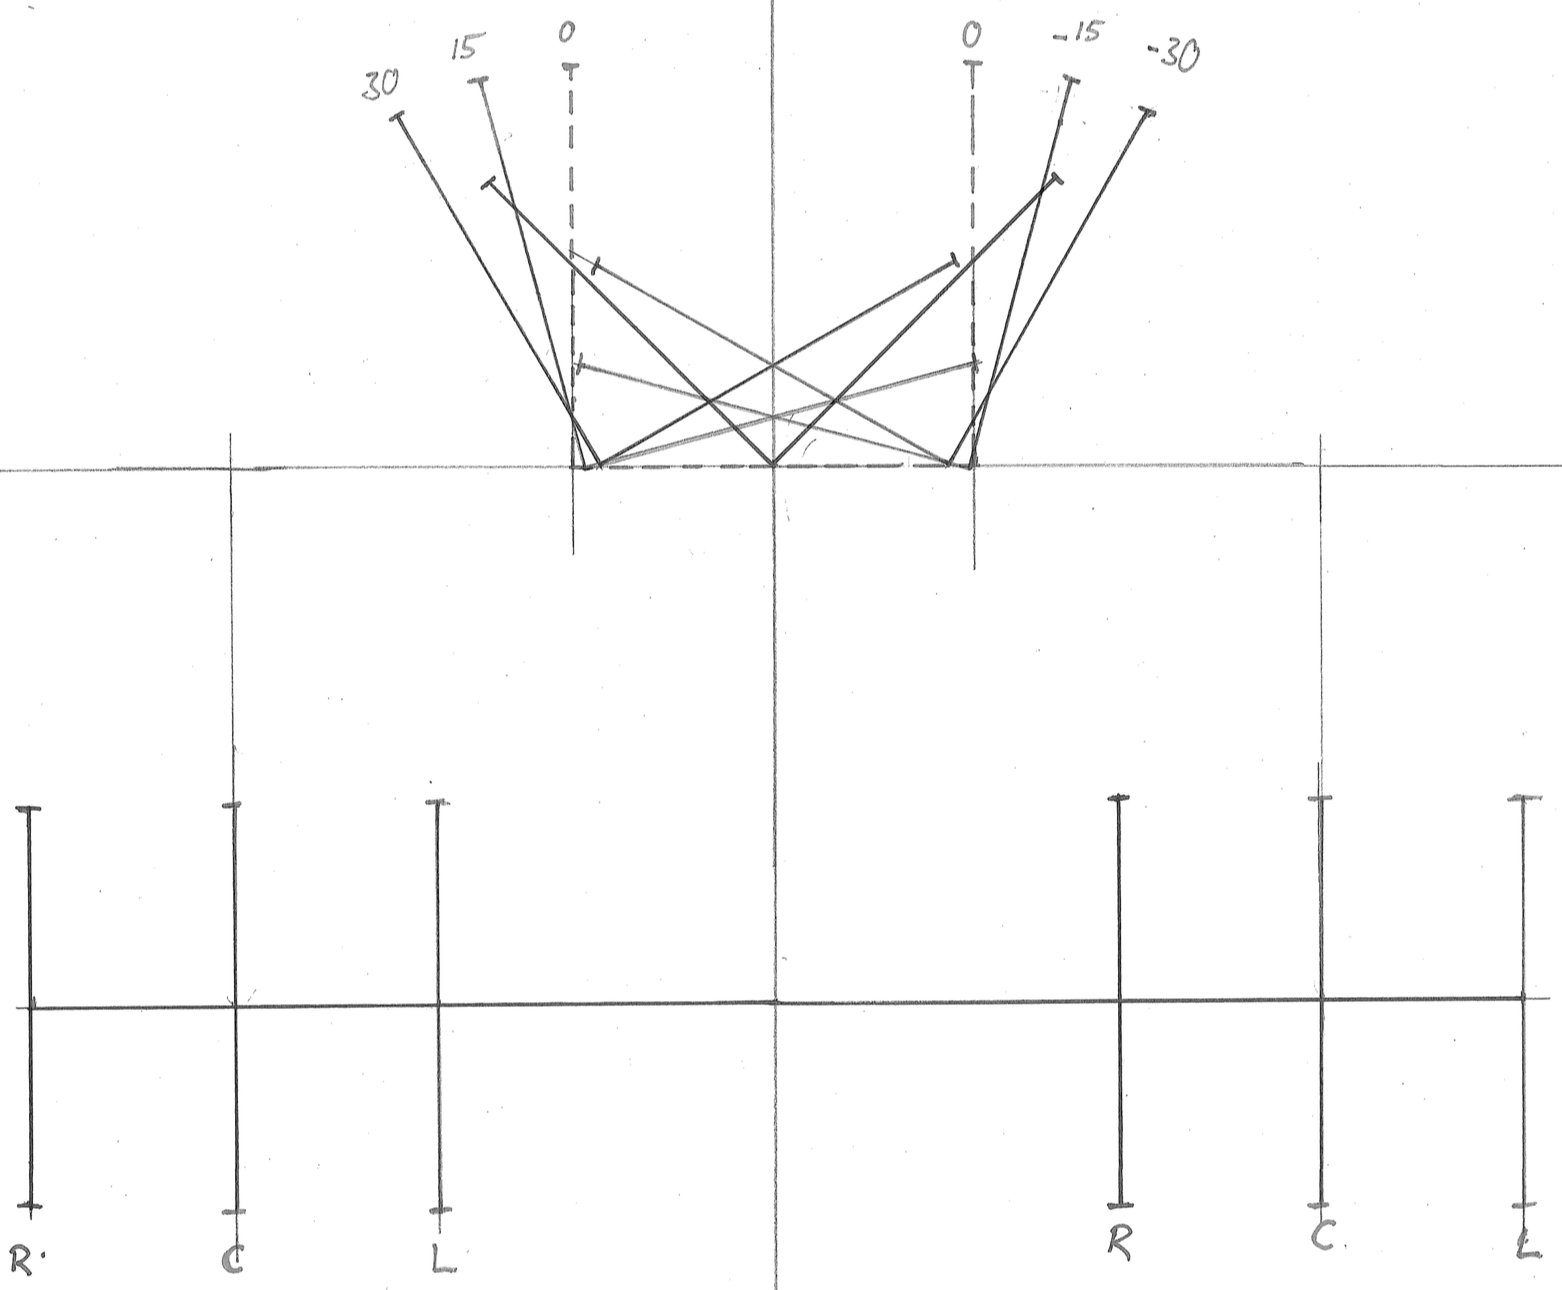
\includegraphics[width=0.7\textwidth]{figures/experiment_plan.png}
	\caption{Evaluation plan with fixed cube poses and starting marks for gripper locations}
	\label{fig:plan}
\end{figure}



\section{Results}

\subsection{Utility of Prior Considerations}

\subsubsection{Action Constraints}
Constraining the action space and preventing the robot from both tossing the block or losing the line of sight has proved useful. While the \texttt{helper} failed several times because of losing the block or succeeded unfairly because of tossing the block actions provided by the \texttt{learner} did not cause this erroneous behavior.

\subsubsection{Demonstrations and Random Exploration}
\figurename~\ref{fig:rho_by_sample} shows the state variable $\rho$ over all samples (time steps of 0.3 seconds) that were collected throughout the whole project. Samples $< 2 \times 10^4$ come from the exclusive \texttt{helper} episodes and show that the pre-defined controller explore this state variable only marginally. This is due to the fact that rotation in the state machine is only done at two places and never to angles $< 0^\circ$ in the state machine.

The following 500 samples stem from keyboard control where exploration of this variable was actively enforced. From $3.5 \times 10^4 - 7.5\times 10^4$, random exploration was enabled. The remaining samples again come from the \texttt{helper} (when it performed the evaluation experiment).


\begin{figure}
	\centering
	\includegraphics[width=0.45\textwidth]{rho_by_sample.eps}
	\caption{Exploration of gripper angles}
	\label{fig:rho_by_sample}
\end{figure}


\subsection{Exploration of States and Actions over Time}
\figurename~\ref{fig:exploration_by_sample} shows how the number of known states and the known state-action pairs evolved over time. Both curves show a steep incline during the keyboard-controlled samples and a similarly steep section during random exploration. Both curves grow linearly, which shows that the state-action space is far from being completely explored.

The number of actions that have been tried in a state decreases logarithmically from the maximum number of actions (ignoring \texttt{HALT}) to the minimum that qualifies a state as known. In a fairly well explored state-action space, the number of known actions per state should be rather equally distributed.

\begin{figure}
\center
    \subfigure{\includegraphics[width=0.45\textwidth]{exploration_by_sample.eps} \label{fig:exploration_by_sample}}
\hfill
    \subfigure{\includegraphics[width=0.45\textwidth]{experience_by_action.eps} \label{fig:experience_by_action}}
\caption{Left: Number of known states (red) and state-action pairs (blue). Right: Number of known actions per state}
\end{figure}


\subsection{Performance Evaluation}
Performance is measured by the number of time steps (0.3 seconds) it took the agent from starting an episode to reaching the goal state. A trial is considered to be timed out if the number of steps is larger than 1000.
Table~\ref{tab:evaluation} summarizes the results of the standardized performance evaluation.

In most cases, the modified controller needs more steps to accomplish the mission than the original one. This a direct consequence from ``discretizing'' the actions and thereby preventing the robot from being very accurate. Examples where the \texttt{helper} is faster than the original controller can occur because of the different goal conditions. The \texttt{cube-mover}'s goal condition was not changed whilst \texttt{helper} is simply stopped when the goal state defined earlier is encountered.

The \texttt{learner} seems very efficient in simpler scenarios as it performs best in all \textbf{Z} experiments and configurations with low angular offset. Higher angular offsets (\textbf{N, P, E}) are often infeasible.

\begin{table}
    \centering
    \caption{Evaluation Results}
    \begin{tabular}{| c | c | c | c |}
        \hline
        Lateral Offset  &   \texttt{cube-mover}   & \texttt{helper}   & \texttt{learner} \\
        \hline
        % 1. Z
        \multicolumn{4}{ c }{\textbf{Z} (angular offset: 0$^\circ$)} \\
        \hline

        %\hline
        %Lateral Offset  &   \texttt{original}   & \texttt{helper}   & \texttt{learner} \\
        \hline
        C & 117 & 324 & \textbf{113} \\
        R & 178 & 465 & \textbf{121} \\
        L & 114 & 730 & \textbf{52} \\
        \hline

        % 2. NL
        \hline
        \multicolumn{4}{ c }{\textbf{NL} (angular offset: -15$^\circ$)} \\
        \hline

        %\hline
        %Lateral Offset  &   \texttt{original}   & \texttt{helper}   & \texttt{learner} \\
        \hline
        C & \textbf{128} & 374 & 234 \\
        R & \textbf{119} & 264 & 236 \\
        L & \textbf{171} & 248 & 658 \\
        \hline
        
        % 3. N
        \hline
        \multicolumn{4}{ c }{\textbf{N} (angular offset: -30$^\circ$)} \\
        \hline
        
        %\hline
        %Lateral Offset  &   \texttt{original}   & \texttt{helper}   & \texttt{learner} \\
        \hline
        C & 284 & \textbf{226} & timed out \\
        R & \textbf{150} & 255 & 233 \\
        L & 254 & \textbf{214} & timed out \\
        \hline

        % 4. PL
        \hline
        \multicolumn{4}{ c }{\textbf{PL} (angular offset: 15$^\circ$)} \\
        \hline
        
        %\hline
        %Lateral Offset  &   \texttt{original}   & \texttt{helper}   & \texttt{learner} \\
        \hline
        C & 161 & 507 & \textbf{96} \\
        R & 215 & 648 & \textbf{130} \\
        L & 178 & 327 & \textbf{79} \\
        \hline

        % 5. P
        \hline
        \multicolumn{4}{ c }{\textbf{P} (angular offset: 30$^\circ$)} \\
        \hline
        
        %\hline
        %Lateral Offset  &   \texttt{original}   & \texttt{helper}   & \texttt{learner} \\
        \hline
        C & \textbf{228} & 531 & timed out \\
        R & 2\textbf{51} & 371 & timed out \\
        L & 180 & 139 & \textbf{92}  \\
        \hline

        % 6. E
        \hline
        \multicolumn{4}{ c }{\textbf{E} (angular offset: 45$^\circ$)} \\
        \hline
        
        %\hline
        %Lateral Offset  &   \texttt{original}   & \texttt{helper}   & \texttt{learner} \\
        \hline
        C & 212 & \textbf{200} & timed out \\
        R & failed & \textbf{224} & timed out \\
        L & \textbf{243} & 637 & timed out \\
        \hline
    \end{tabular}
    \label{tab:evaluation}
\end{table}


\section{Discussion}

%\begin{itemize}
%    \item Convergence for Q-Learning nearly impossible here
%    \item Was the state representation useful?
%\end{itemize}

\subsection{Project Goals}

\subsubsection{Goal: Online learning}
The developed software implements a simple learning algorithm. When the robot acts, new data samples are available and are immediately integrated into the learning. Being able to run the learning algorithm on the robot itself without having to transfer the data to an external device became one of the major goals after the first steps in this project. There are no problems regarding timing or memory so far.

\subsubsection{Goal: Improve learned behavior}
The positive examples in Table~\ref{tab:evaluation} where the \texttt{learner} reaches the goal significantly faster than both other controllers seem very promising but on the other hand the learned behavior seems incapable of transferring this knowledge to more complex situations. In the \textbf{E}-configurations it even starts to oscillate, which is somehow obvious because both trajectories left and right might seem equally to the robot.

When looking at the complete task of approaching to and aligning with an object, this could not be significantly improved yet. Making the restriction to small angular offsets would allow to speak of an improvement. However, this performance cannot be considered stable. 

\subsubsection{Goal: Simplification of controller development}
Given that only a very little part of the state-action space has been explored, it is hard to tune the learning algorithm itself meaning parameters like learning rate $\alpha$ and discount factor $\gamma$. This also complicates the development of controllers for other tasks.

Data collection is the most difficult part here as no simulations are available and one has to deal with hardware problems and especially with time.

In this particular case, the underlying controller already seems very robust. It is remarkable that even removing all the precision it used in the original \texttt{cube-mover} did not prevent it from reaching the goal in the end.

\subsection{Suitability of Q-Learning}
We noticed that our learning algorithm only managed to produce good policies for very simple configurations (e.g. starting straight and close to the block). For configurations with lateral or angular offsets, the robot nearly never succeeded within 20 minutes. One possible reason is that Q-learning might not be a suitable solution for our goal. Q-learning is known to converge to the optimal solution very slowly. In our case, we are facing a huge number of possible state-action pairs. After all of our experiments, we have only seen about 5\% of the states yet. With simple Q-learning the time for convergence will be very long. Consider the following example:

Assume the agent is on its way to reaching the goal on a suboptimal (but already learned) way. In some state $s_1$, it starts to explore a different plan (by doing a random action $a_1$). Let's say the current $Q(s_1, a_1)$  is very low because the cube is further away and also the following state is not known (i.e. $Q(s_2, a_{max})$ is only the initialization value, which is 1 at the moment). Consequently, for $s_1$: $Q(s_1, a_1) < Q(s_1, a_{max})$ and therefore, when $s_1$ is encountered next time, $a_1$  will only be chosen if random exploration happens to be occur again and also $a_1$ is the random action chosen out of the 8 available actions.

Assume, it turns out that this this subtle change of actions ($a_1$ instead of the current $a_{max}$) results in a much better way of reaching the goal. Then, the agent has clearly explored a better strategy. 
Assume the new strategy took $N$ steps from $s_1$ to the goal and say the exploration goes through $N$ new states on the way to the goal. Then, all the new Q-values are carrying the initialization value and only the Q-value directly before the goal is very high, i.e. $Q(s_{goal - 1}, a_{max})$.
However, Q-values do not propagate back immediately but only when the state-action pair occurs the next time. In order to propagate this new finding back to $s_1$ the agent would have to follow the same strategy another $N$ times until the benefit of $a_1$ becomes evident in $s_1$ (which would make the non-exploring agent in $s_1$ decide for $a_1$, i.e. $a_{max} = a_1$).

\subsection{Suitability of the Reward Function}
Knowing that spreading rewards throughout the whole state space can facilitate the learning procedure compared to problems where reward is only given at the goal state, our reward function was supposed to constantly give reward depending on the action quality. Our reward function is not convex and cannot encode the distance to the goal state. Given that there is only one goal, both are risks that might make the learning algorithm getting stuck in local optima.

The simplest options for a reward function that does not bring up that risk is to give zero reward at all states that are no goal states and some high reward at the goal state. In this case, the learning boils down to a graph search problem where action-values encode the distance to the goal. The same is true for giving zero reward at the goal state and giving a constant negative reward for doing any action. Then, the problem can be formulated as cost minimization. Both of these options require a good knowledge of the state-action space, which is currently not given in our case.

\subsection{State Generalization}
One last difficulty is how to leverage learned knowledge in unseen situations by generalizing from know states. In this work, generalization was done by looking for nearby states. Nearby was interpreted in a Hamming distance like manner meaning that states that have small differences in their state variables are considered close. A potential problem resulting from this is that two states that seem close in this sense are not equally close to the goal state and might require two completely different actions to proceed. For the purpose of exploration, however, this approach seems appropriate.

%\begin{itemize}
%    \item What has been achieved wrt the goal?
%    \item Promising alternatives to Q-learning
%    \begin{itemize}
%        \item Tiling: shrink state space
%        \item Switch to model-based learning and use state factorization
%    \end{itemize}
%\end{itemize}

\chapter{Outlook and Summary}

\section{Outlook}
Performing task learning with the MarXbot has proved difficult due to the complexity of its action space and to time consuming data collection. Nevertheless, there exist remedies to still apply learning algorithms to the MarXbot successfully.

\subsubsection{Online to offline learning}
For future work dealing with learning on the physical robot, the requirement of online learning should be turned down. With the simplest form of Q-learning it takes very long for a new experience to propagate back to a state where it would change the policy. As the number of states encountered in an episode is tiny compared to the whole state space, new encounters won't change the policy much during a single episode. Therefore online learning can be replaced by offline learning without any disadvantages.

\subsubsection{Model-based methods}
Model-free methods like Q-learning tend to be sample inefficient while model-based methods are more sample efficient, meaning that they leverage samples better and gain more knowledge. A model consists of a state transition table and the respective probabilities as well as the expected rewards. Updating the model after each episode would ensure that all the new experience is completely reflected in the model (i.e. the current memory). Additionally, this would also eliminate problems with reward function design because one could simply use one of the primitive ideas mentioned above.

\subsubsection{State factorization}
The remaining problem would still be how to transfer knowledge from known states to unseen ones. Hester \cite{hester2009generalized} presented a promising solution to this. Assuming that changes in the individual state variables are statistically independent and assuming that modeling these changes requires less complexity than modeling the exact state space, the model can be approximated by other learning methods. Hester argued that decision trees are appropriate for this purpose.

A factorized model representation becomes particularly appealing to the MarXbot because unseen states and also their approximate values can be drawn from this model. Sample efficiency is increased even more and there is a bigger chance to explore the huge state space that we are given here.

To support this promising idea, histograms of the relative changes of the four state variables used in this work are shown in Figures~\ref{fig:d_smin_x}, \ref{fig:d_smin_y}, \ref{fig:d_rho} and \ref{fig:d_line}. The underlying data are again the $\sim$120000 samples collected from all the episodes before evaluating the \texttt{learner}.

In the 99\% confidence interval, i.e. 99\% of the data lie within that range, the values to be considered for the model are: $\Delta s_{min_x} \in [-3, 3]$, $\Delta s_{min_y} \in [-2, 2]$, $\Delta line \in [-5, 5]$, $\Delta \rho \in [-2, 2]$. The fact that the range of $\Delta line$ spans more than the range of $line$ is either due to the fact that the sign of the line switches frequently when the cube is centered and either almost aligned or close to 45$^\circ$ off, or it shows that this variable is inadequate.

If we additionally use a primitive reward function (that does not require its own model) the total number of nodes in the decision trees is approximately $6\times10^4$.

\begin{figure}
\center
    \subfigure{\includegraphics[width=0.45\textwidth]{d_smin_x.eps} \label{fig:d_smin_x}}
\hfill
    \subfigure{\includegraphics[width=0.45\textwidth]{d_smin_y.eps} \label{fig:d_smin_y}}
\caption{Relative change in $s_{min_x}$ (left) and $s_{min_y}$ (right)}
\end{figure}

\begin{figure}
\center
    \subfigure{\includegraphics[width=0.45\textwidth]{d_rho.eps} \label{fig:d_rho}}
\hfill
    \subfigure{\includegraphics[width=0.45\textwidth]{d_line.eps} \label{fig:d_line}}
\caption{Relative change in $\rho$ (left) and $line$ (right)}
\end{figure}


\section{Summary}
The concept of a simple learning algorithm, Q-learning, has been applied to the MarXbot in order to improve the behaviors needed to approach and align with an object. Based on the original controller, two controllers were developed in Aseba. One imitating the original controller but with a massively smaller set of actions and another one allowing the combination of manual control, control from learned behaviors and control through the modified version of the original controller. A framework for data collection learning and acting based on learned knowledge was developed in Python.

Experiments of a total duration of more than eleven hours were conducted to explore the state space and produce Q-tables from this experience. Nevertheless, only a fraction of this space is known to our learner at this point and it keeps learning with every new experiment.

In the evaluation, our learned policy could not clearly outplay the existing controllers. Due to various reasons, this result must be seen as intermediate. Several options to improve learning on the MarXbot are available and need further investigation.


%\end{document}
